\documentclass[aspectratio=169]{beamer}

% 中文支持
\usepackage[UTF8]{ctex}

% 数学相关宏包
\usepackage{amsmath,amssymb,enumerate}

% PPT 主题
\usetheme{Madrid}

% 字体设置
\setCJKmainfont{KaiTi}
\setCJKsansfont{KaiTi}
\setCJKmonofont{KaiTi}
\title{这就是开源}
\subtitle{第二讲：Git与Github}
\author{潘宇琦\hspace*{1em}申鹏威}
\begin{document}

\begin{frame}
	\title{这就是开源}
	\subtitle{第二讲：Git与Github}
	\author{潘宇琦\hspace*{1em}申鹏威}
	\date{2026年11月}
	\titlepage
\end{frame}	
	
\begin{frame}{回顾上一讲}
\begin{block}{如何协作？}
	\hspace*{2em}在上一讲中，我们认识了操作系统的发展历史，什么是开源以及开源的意义。但现在仍然面临一个问题：当我们真正开始接触开源时，如何高效地参与开源项目、管理代码，以及与其他开发者协作？
	
	\hspace*{2em}我在上一讲提到开源之所以发展得如此迅速是因为计算机的普及和互联网的发展，但是仅仅依靠这两点还是不够的。我们需要一个强力的工具，这个工具就是Git。
\end{block}
\end{frame}	

\begin{frame}{Git的前世今生}
\begin{block}{最初}
	\hspace*{2em}最开始开发Linux的时候，大家交流代码提交补丁主要是依靠电子邮件，然后林纳斯把通过测试的补丁放到自己维护的代码树中，最终由林纳斯推出整个代码树的新版本，如果想查看新版本做了哪些改进，只能使用diff这一个工具，非常的不便。
\end{block}
\begin{block}{版本控制系统(Version Control System，VCS)}
	\hspace*{2em}一种用于记录文件或项目随时间发生的变化，并对这些变化进行管理的工具。
	\begin{itemize}
		\item 记录每一次修改
		\item 查看不同版本之间的差异
		\item 恢复到过去的某个版本
		\item 追踪修改者以及修改原因
		\item 协调多个开发者共同开发项目
	\end{itemize}
\end{block}
\end{frame}

\begin{frame}{Git的前世今生}
\begin{block}{Git诞生}
	\begin{itemize}
		\item 2002 年，Linux 内核开发团队开始使用一款名为 BitKeeper 的商业分布式版本控制系统。当时该软件允许 Linux 社区免费使用。
		\item 2005 年，BitKeeper 公司与 Linux 内核开发社区发生矛盾，Linux 社区失去了免费使用 BitKeeper 的权利。
		\item Linus Torvalds 决定自己开发一套版本控制系统，以满足 Linux 内核的大规模协作需求。
		\item 2005 年 4 月 7 日，Git 的第一个提交诞生。此后，Git 逐渐发展成为今天广泛使用的版本控制系统。
	\end{itemize}
\end{block}
\begin{block}{BitKeeper后来：}
	\hspace*{2em}于2016年宣布开源，使用Apache 2.0许可证，于2020年停止开发。
\end{block}
\end{frame}
	
\begin{frame}{如何安装Git}

\end{frame}

\begin{frame}{Git 的基本工作原理}
\begin{block}{仓库}
	\hspace*{2em}当我们在一个项目文件夹中执行 `git init` 命令时，Git 会在该文件夹下创建一个名为 `.git` 的隐藏目录，用于保存版本控制所需的信息。此时，该文件夹就成为了一个 Git 仓库。
	
	\hspace*{2em}需要注意的是，Git 并不要求初始化的文件夹必须为空，原有文件也不会受到影响。
\end{block}
	\centering
	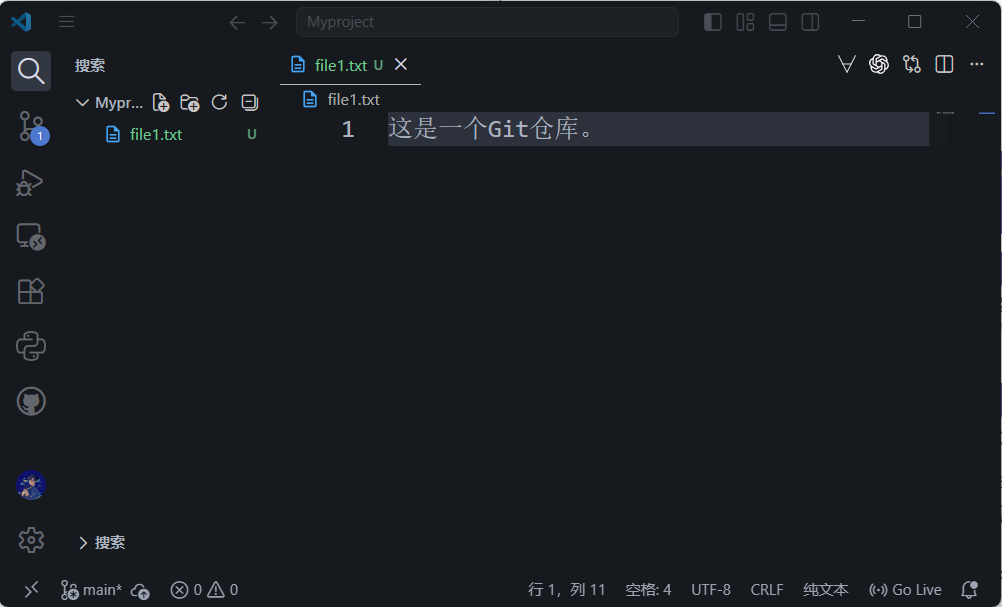
\includegraphics[width=0.507\textwidth,keepaspectratio]{images/1.png}
\end{frame}

\begin{frame}{Git 的基本工作原理}
	\begin{block}{.git文件夹}
		\hspace*{2em}这个文件夹在被初始化为仓库之后，就会增加一个名为.git的隐藏文件夹，其中会含有版本控制的重要信息。
	\end{block}
	\centering
	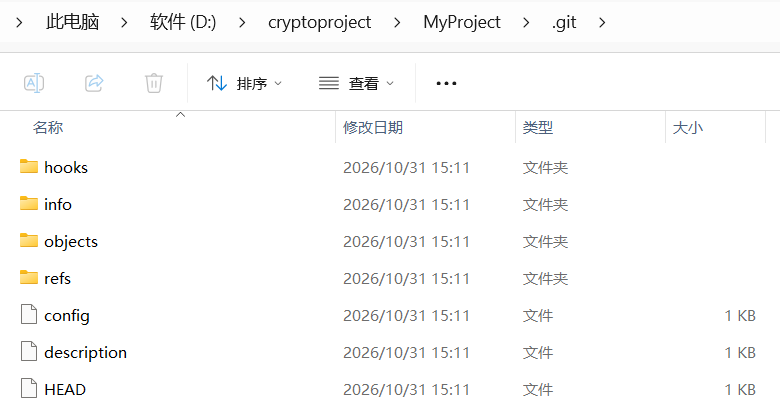
\includegraphics[width=0.507\textwidth,keepaspectratio]{images/2.png}
\end{frame}	

\begin{frame}{Git 的基本工作原理}
\begin{block}{工作区}
	\hspace*{2em}我们实际看到和编辑的项目文件。对文件进行修改、创建和删除，都是在这里完成的。
\end{block}
	\centering
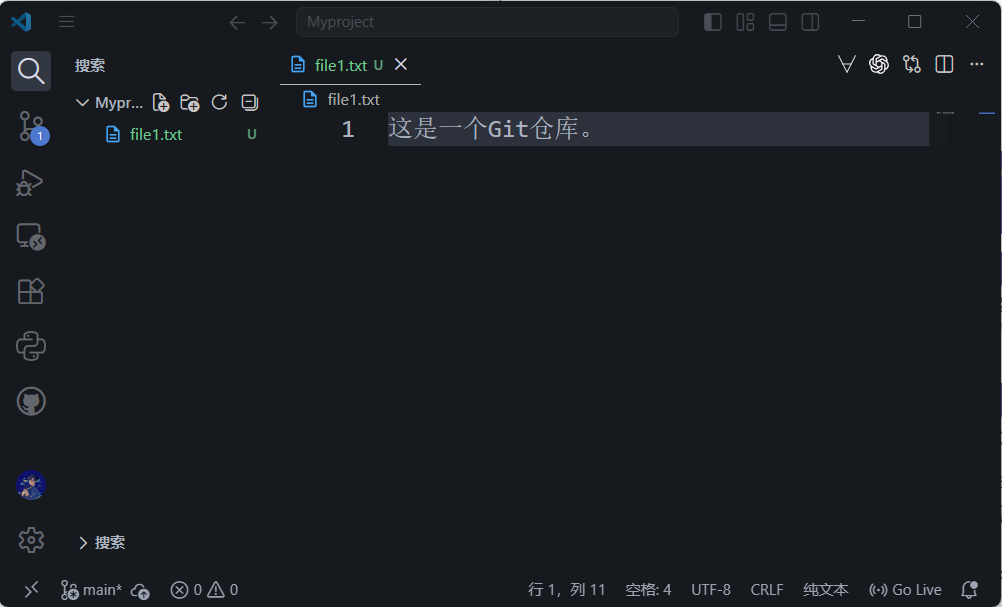
\includegraphics[width=0.507\textwidth,keepaspectratio]{images/1.png}
\end{frame}

\begin{frame}{Git 的基本工作原理}
\begin{block}{暂存区}
	\hspace*{2em}我们使用git add 命令把修改过或者新创建或者删除过的文件提交到暂存区。暂存区不像工作区一样直接可见，其具体信息会被保存在.git文件夹中。
\end{block}
\centering
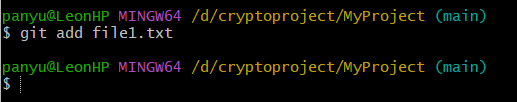
\includegraphics[width=0.507\textwidth,keepaspectratio]{images/3.png}	
\end{frame}

\end{document}